\chapter*{Introducción}\label{chapter:introduction}
\addcontentsline{toc}{chapter}{Introducción}



El Estado cubano pide dinero prestado a entidades de la econom\'ia a trav\'es del Banco Central de Cuba. El monto solicitado y el inter\'es m\'aximo con el que se devolver\'a se plasman en un documento llamado bono soberano.  Los posibles prestamistas participan en una subasta por el bono y el que menor tasa de inter\'es exija por el pr\'estamo ser\'a el ganador, y el Estado pasar\'a a ser su prestatario.  Para decidir qui\'enes participan en la subasta, se confeccionan los Comit\'es de Mercado Financiero (CMF).  Los miembros y el presidente de cada Comit\'e se deciden mediante un proceso electoral en el que cualquier elector puede ceder su poder de voto a otro elector. A ese tipo de elecci\'on el autor le denomina \textbf{votaci\'on representativa}.  


En un sistema de votaci\'on representativa  los votos se transfieren, esto es, si una persona $A$ vota por una persona $B$ y esta, a su vez, vota por  $C$, entonces el voto de $A$ se transfiere a $C$. En el caso particular de la confecci\'on de los CMF, cada individuo puede votar por a lo sumo otra persona.

La figura \ref{fig:r-voting} ilustra un ejemplo de votación en el que $A$ votó por $B$, $B$ y $E$ votaron por $C$ y $C$ votó por $D$. $B$ obtiene solamente el voto de $A$, mientras que $C$ obtiene los votos de $A$, $B$ y $E$. $D$ recibe el voto directo de $C$ y, con este,  los votos indirectos de los restantes participantes.

\begin{figure}[h]
    \centering
    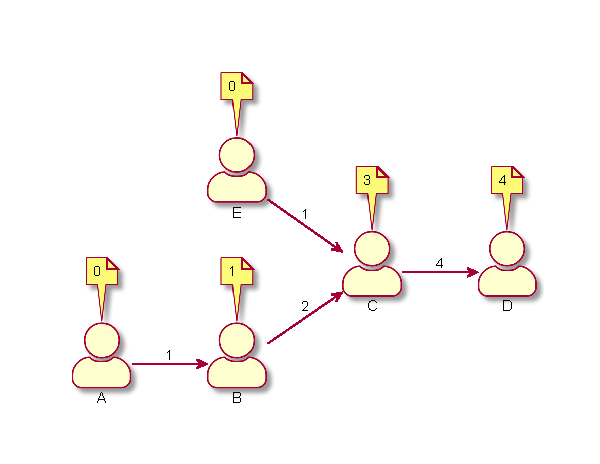
\includegraphics{Graphics/rep-voting.pdf}
    \caption{Conteo de votos en votación representativa.}
    \label{fig:r-voting}
\end{figure}

En un proceso electoral de este tipo pueden surgir ciclos de votación, como el que se muestra en la figura \ref{fig:voting-cycle}, donde el voto emitido por $D$ hacia $B$ forma un ciclo que los involucra a ambos y a $C$. En tal caso, no queda claro cu\'antos votos otorgarle a las personas involucradas en el ciclo.  Uno de los objetivos del presente trabajo es \textbf{dise\~nar e implementar una asignaci\'on justa de  votos para los electores involucrados en un ciclo de votación}. 

\begin{figure}[h]
    \centering
    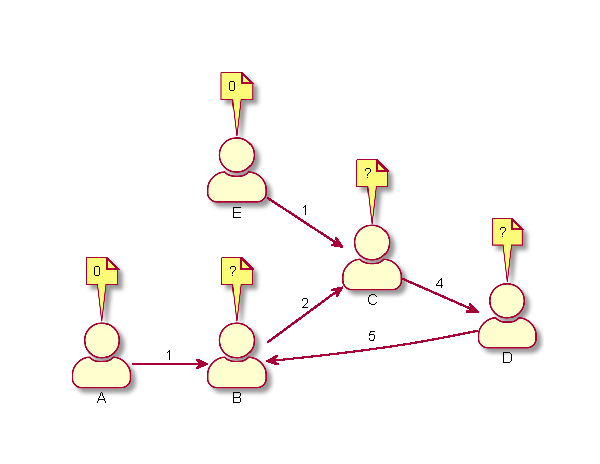
\includegraphics{Graphics/voting-cycle.pdf}
    \caption{Ciclo de votaci\'on.}
    \label{fig:voting-cycle}
\end{figure}

Para seleccionar un presidente para un CMF, se realiza una elecci\'on representativa y el que obtenga la mayor cantidad de votos es el ganador. Puede pasar que m\'as de una persona obtenga la mayor cantidad de votos.   Esto no es deseable, ya que el presidente debe ser \'unico. En este sentido, otro de los objetivos de este trabajo es \textbf{dise\~nar e implementar un mecanismo de desempate}.

% pa mantener un sistema distribuido de goquorum es necesario al menos 4 nodos % @NOTE chekea eso 

Tradicionalmente en estas elecciones, como en muchas otras, los votos son emitidos en boletas de papel y el conteo es realizado manualmente. Esto puede traer consigo ciertos problemas que causan desconfianza en el electorado, como son los votos falsos y el mal conteo de los votos.   Si no se hace una verificaci\'on rigurosa de la identidad del votante, entonces se puede emitir votos con relativa facilidad en nombre de personas que no han votado (votos falsos). Si el conteo no est\'a supervisado adecuadamente, pueden surgir errores en los resultados, ya sea por intereses personales o errores humanos.

En un sistema de votaci\'on electr\'onico se  pueden lograr diversas formas de verificaci\'on biom\'etrica, por ejemplo, mediante la huella digital o el esc\'aner ocular. Por otro lado, en estos sistemas se puede contar los votos de manera eficiente mientras se van realizando y se  puede publicar en vivo los resultados. 

Otras bondades poseen los sistemas electrónicos, como son la flexibilidad, lo fácil que pueden ser de usar y lo baratos que resultan con respecto a los sistemas tradicionales. Sin embargo, muchos de los sistemas electrónicos existentes son centralizados, esto es, dependen de que una agencia central se encargue de registrar, manejar, calcular y revisar los votos. Toda la confianza debe entonces ser depositada en esa agencia, lo cual hace vulnerable al sistema.
 
Un sistema digital descentralizado de votación no tiene ese problema. Una de las tecnologías descentralizadas empleadas actualmente es \textit{blockchain}.   \textit{Blockchain} es un registro distribuido e inmutable  de transacciones. Lo que se transacciona puede ser tangible, como son  una casa o dinero en efectivo, o intangible, como son el derecho de autor de una obra o el voto de un elector por un candidato (\cite{blockchain-ibm}). La inmutabilidad y seguridad de este registro se basan en principios de  criptografía, descentralizaci\'on y mecanismos de consenso (\cite{blockch-security-ibm}). 


% Hacerlo con \textit{blockchain} ta bueno xq resuelve la parte m\'as importante de esos problemas. 

Desde el surgimiento de Ethereum se puede implementar comportamientos complejos mediante contratos inteligentes. Ethereum es una plataforma \textit{blockchain} que establece una red p\'ublica que ejecuta y verifica c\'odigo de manera segura. A dicho c\'odigo o al programa que resulta de ejecutarlo se le conoce como contrato inteligente (\cite{eth-aws}).  

No es deseable que el proceso electoral en el CMF se realice en una red p\'ublica, ya que es un proceso que s\'olo concierne a las partes involucradas. Por otro lado, desplegar un contrato inteligente en Ethereum puede costar miles de d\'olares (\cite{eth-deploy}). Estos dos factores hacen que no sea factible realizar la implementaci\'on de este trabajo sobre la red p\'ublica de Ethereum. 

GoQuorum es una implementaci\'on de Ethereum capaz de crear redes privadas y con mecanismos de autorizaci\'on. En GoQuorum tambi\'en se puede personalizar el costo del despliegue de los contratos inteligentes, incluso, puede hacerse nulo. Por todo lo dicho anteriormente, GoQuorum es una buena opci\'on en la que implementar el sistema de votaci\'on representativa del CMF.


Existen implementaciones de sistemas de votaci\'on en otras \textit{blockchain} (\cite{agora}) y tambi\'en en Ethereum (\cite{ovn} y \cite{borda_count}), pero no se conoce ninguna implementaci\'on de un sistema de voto representativo en GoQuorum.

\todo[inline, disable]{@TODO decir que el Instituto de Criptograf\'ia implement\'o un sistema de votaci\'on en hyperledger fabric pero tampoco nos sirve. ?`C\'omo cito eso?}

En \cite{wang2017review} se proponen los requisitos principales y opcionales que debe cumplir todo sistema de votaci\'on electr\'onico. Entre ellos est\'an:
\begin{itemize}
    \item correctitud: los votos deben ser contados correctamente, esto es, todos los votos v\'alidos deben ser contados y los votos inv\'alidos no deben ser contados.

    \item privacidad: no se conoce la decisi\'on del votante.

    \item prevenci\'on del doble voto: un votante no puede emitir la misma boleta dos veces. También se debe evitar que un tercero pueda clonar una boleta previamente emitida por un votante, para registrarla de nuevo a nombre de ese votante.

    \item elegibilidad: s\'olo los votantes autorizados pueden votar.

    \item robustez: poder lidiar con una cierta cantidad de comportamientos incorrectos por parte de los votantes o con una falla parcial del sistema.

    \item justeza: no se calculan los resultados hasta el fin de la votaci\'on.

\end{itemize}

Con el presente trabajo de diploma  se pretende dise\~nar e implementar un sistema de votaci\'on representativa en GoQuorum que cumpla con los requisitos mencionados anteriormente. El sistema debe ser capaz, adem\'as, de realizar elecciones para un CMF, asignando un valor justo de votos para los electores involucrados en un ciclo de votaci\'on y determinando un ganador, incluso cuando hay empate en el primer lugar. El sistema debe ser lo m\'as gen\'erico posible, de forma tal que sea factible su uso m\'as all\'a del entorno bancario.




% estudiar, disenyar y modelar, implementar y evaluar resultados

% @TODO decir d q' va cada capi'tulo

% @NOTE habla en tiempo presente, 3ra persona del singular, e.g. "el autor ha desarrollado", "el autor ha realizado", etc.